% !TEX root = ../core/tetelfuzet.tex

\section{Definiálja a racionális szám fogalmát!}
\label{009}

\begin{defin}[Természetes számok]
Az egyet és annál nagyobb számokat összefoglaló néven \dashuline{természetes
számok}nak hívjuk, a természetes számok halmazának jele $\Naturals$. Azaz:
\[
  \Naturals \coloneqq \{1; 2; 3; 4; 5; \dots{ }\}
\]

Tulajdonságai: az $\Naturals$ (\hunquote{naturalis}, latinul am.
\hunquote{természetes}) halmaz
\begin{itemize}
\item az összeadásra és szorzásra nézve zárt
\item a halmaz rendezett
\item végtelen sok elemet tartalmaz
\end{itemize}

A $0$-val bővített természetes számok halmazát $\Naturals_0$ jelöli. Tehát
$\Naturals_0 \coloneqq \Naturals \cup \{0\}$
\end{defin}

\begin{defin}[Egész számok] ($\Naturals$ bővítése)
Azokat a számokat, amelyek felírhatóak két természetes szám különbségeként
\dashuline{egész számok}nak nevezzük. Az egész számok együttesen az egész
számok halmazát alkotják, melynek jele $\Integers$. Azaz:
\[
  \Integers \coloneqq \{n | \exists a, b \in \Naturals:  n = a - b\}
\]

(Megjegyezzük, hogy $a, b \in \Naturals_0$ esetén a fent megadottal ekvivalens
halmazt kapunk).

Tulajdonságai: a $\Integers$ (\hunquote{zahlen}, németül am.
\hunquote{számolni}) halmaz
\begin{itemize}
\item az összeadásra, szorzásra és kivonásra nézve zárt
\item a halmaz rendezett
\item végtelen sok elemet tartalmaz
\end{itemize}
\end{defin}

\begin{defin}[Racionális számok] ($\Integers$ bővítése)
Azokat a számokat, amelyek felírhatóak két egész szám hányadosaként, ahol a
nevező nullától különböző, \dashuline{racionális számok}nak nevezzük. A
racionális számok együtt a racionális számok halmazát alkotják, melynek jele 
$\Rationals$. Azaz:
\[
  \Rationals \coloneqq \Big\{x |\exists a, b \in \Integers, b \neq 0:
  x = \dfrac{a}{b}\Big\}
\]

Tulajdonságai: a $\Rationals$ (\hunquote{qoutiens}, latinul am.
\hunquote{hányszor}) halmaz
\begin{itemize}
\item a négy alapműveletre nézve zárt
\item a halmaz rendezett
\item végtelen sok elemet tartalmaz
\end{itemize}
\end{defin}

\begin{theorem2}[Racionális számok tizedestört alakja]
\label{theorem:racfrac}
Minden racionális szám felírható véges vagy végtelen szakaszos tizedestört
alakban.
\end{theorem2}

\begin{theoremconv2}
\label{theorem:racfracconv}
Minden véges vagy végtelen szakaszos tizedestört felírható két egész szám
hányadosaként, tehát racionális szám.
\end{theoremconv2}

\begin{proof5}
A tétel és megfordítása bizonyításától eltekintünk.
\end{proof5}

\begin{theorem4}
A tizedestört alak korlátozottan egyértelmű, ugyanis bizonyítható, hogy a
végtelen sok $9$-esre végződő tizedestörteknek van másik alakjuk, amit úgy
kapunk, ha a $9$-esek előtti tizedesjegyet eggyel növeljük, és a $9$-esek
helyére $0$-át írunk, például:
$\dfrac{3}{4} = 0,75 = 0,7500000\dot{0} = 0,7499999\dot{9}$
\end{theorem4}

\begin{proof5}
A tétel bizonyításától eltekintünk.
\end{proof5}

\begin{note}[Racionális számok tört alakjai]
Minden racionális szám végtelen sok módon adható meg
$\dfrac{a}{b}\;\;(b \neq 0)$ alakban. Egy adott racionális szám különböző
alakjai egymásból egyszerűsítéssel illetve bővítéssel nyerhetőek.
\end{note}

\begin{note}[Racionális számok ábrázolása]
A racionális számokat számegyenesen ábrázoljuk, ahol minden racionális számnak
megfelel egy pont, de nem minden pontnak felel meg racionális szám.
\end{note}

\begin{defin2}[Irracionális számok]
Azokat a számokat, amelyek nem írhatóak fel két egész szám hányadosaként, ahol
a nevező nem nulla, \dashuline{irracionális számok}nak nevezzük. A irracionális
számok együtt a irracionális számok halmazát alkotják, melyet jelölhet 
$\Irrationals$, vagy $\mathbb{I}$ (a félreértések elkerülése végett szokás még
$\Reals\backslash\Rationals$-ként, tehát \hunquote{nem racionális valósként}
hivatkozni rájuk). Azaz:
\[
  \Irrationals \coloneqq \Big\{x | \nexists a, b \in \Integers, b \neq 0 :
  x = \dfrac{a}{b}\Big\}
\]

Tulajdonságai: az $\Irrationals$ halmaz
\begin{itemize}
\item a halmaz rendezett
\item kontinuum (megszámolhatatlanul végtelen) sok elemet tartalmaz
\end{itemize}
\end{defin2}

\begin{theorem2}[Irracionális számok tizedestört alakja]
\label{theorem:irracfrac}
Minden irracionális szám felírható végtelen nem szakaszos tizedestört alakban.
\end{theorem2}

\begin{theoremconv2}
\label{theorem:irracfracconv}
Egy végtelen nem szakaszos tizedestört nem írható fel két egész szám
hányadosaként, tehát irracionális szám.
\end{theoremconv2}

\begin{proof5}
A tétel és megfordítása bizonyításától eltekintünk.
\end{proof5}

\begin{note2}[Irracionális számok ábrázolása]
A irracionális számokat számegyenesen ábrázoljuk, ahol minden irracionális
számnak megfelel egy pont, de nem minden pontnak felel meg irracionális szám.

Irracionális szám például a $\sqrt{2} \approx 1,4142$, a $\pi \approx 3,1415$
és az $e \approx 2,7182$.
\end{note2}

\begin{defin2}[Valós számok]
\label{def:real}
Azokat a számokat, amelyek racionálisak vagy irracionálisak \dashuline{valós
számok}nak nevezzük. A valós számok együtt a valós számok halmazát alkotják,
melynek jele $\Reals$. Azaz:
\[
  \Reals \coloneqq \{x | x \in \Rationals \cup \Irrationals\}
\]

Tulajdonságai: az $\Reals$ (\hunquote{realis}, latinul am. \hunquote{valós})
halmaz
\begin{itemize}
\item a négy alapműveletre nézve zárt
\item a halmaz rendezett
\item kontinuum (megszámolhatatlanul végtelen) sok elemet tartalmaz
\end{itemize}
\end{defin2}

\begin{theorem2}[Valós számok tizedestört alakja]
Minden valós szám felírható véges, végtelen szakaszos vagy végtelen nem
szakaszos tizedestört alakban.
\end{theorem2}

\begin{theoremconv2}
Egy véges, végtelen szakaszos vagy végtelen nem szakaszos tizedestört  valós
szám.
\end{theoremconv2}

\begin{proof2}
A tétel és megfordítása triviálisan következik \atold\ref{def:real}+es{}
definícióból és \aref{theorem:racfrac}, \ref{theorem:racfracconv},
\ref{theorem:irracfrac}, \told\ref{theorem:irracfracconv}+es{} tételekből.
\end{proof2}

\begin{note2}[Valós számok ábrázolása]
A valós számokat számegyenesen ábrázoljuk, ahol minden valós számnak megfelel
egy pont, és minden pontnak megfelel egy valós szám.
\end{note2}

\begin{note2}[A számhalmazok egymáshoz való viszonya]
Megállapítható, hogy:
$\Naturals \subset \Integers \subset \Rationals \subset \Reals$

\begin{figure}[!h]
	\centering
	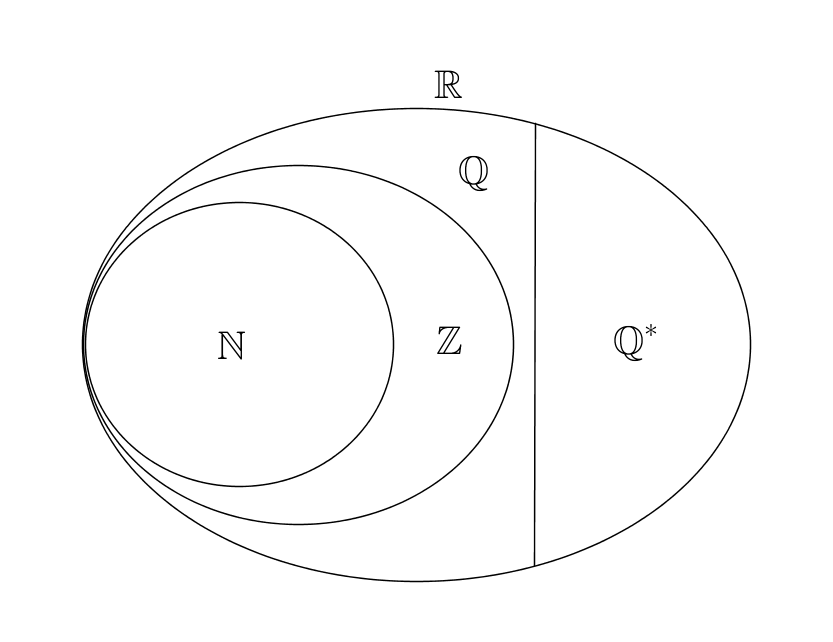
\includegraphics[height=4cm]{../images/009_sets_of_numbers}
	\caption{Számhalmazok Venn-diagramon} 
	\label{fig:numberset}
\end{figure}
\end{note2}

\begin{note4}[Végtelen számok]
Azt a számot, ami nagyobb minden valós számnál szokás pozitív végtelennek
nevezni és $+\infty$-nel (vagy csak $\infty$-nel, ha ez nem okoz félreértést)
jelölni. Azt a számot, ami kisebb minden valós számnál szokás negatív
végtelennek nevezni és $-\infty$-nel jelölni. Szokás definiálni a
\hunquote{végtelenekkel kiegészített valós számok halmazát} a következőképpen:
$\overline{\Reals} \coloneqq \Reals \cup \{-\infty; +\infty\}$
\end{note4}

\begin{note2}[Negatív/Pozitív részhalmazok]
A számhalmazok negatív/pozitív részhalmazait szokás felső indexbe tett $-$/$+$
jellel jelölni. Azaz például $\Integers^-$ jelentése \hunquote{a nullánál
kisebb egész számok halmaza}, míg $\Reals^+$ jelentése \hunquote{a nullánál
nagyobb valós számok halmaza}. Érdekesség, hogy $\Integers^+ \equiv \Naturals$,
míg $\Integers \backslash \Integers^- \equiv \Naturals_0$.
\end{note2}

\textbf{Lásd még:} \ref{004}
